\documentclass{beamer}
\usetheme{Boadilla}

\title{Autonomous Vehicles and Artificial Intelligence Lab}
\subtitle{Final Presentation - Buggy Busters}
\author{
	K. L.
	\and
	N. O.
	\and
	J. D.
	\and
	A. A.
}
\institute{Ruhr University Bochum}
\date{\today}

\begin{document}



\begin{frame}
	\titlepage
\end{frame}

\begin{frame}
	\frametitle{Introduction}
	\begin{itemize}
		\item F1Tenth car platform: implements basic functionality
		\begin{itemize}
			\item driving \& steering
			\item nodes for fetching \& publishing sensor \& transform data
		\end{itemize}
		\item basic manuals for car platform \& software stacks
		\item Gazebo Fortress: SDF file for F110th standard in order for simulation being as close as possible to real-world
		\item hardware: 4 wheel drive, Ackermann steering, IMU, depth camera, RGB camera, \& LiDAR
	\end{itemize}
\end{frame}

\begin{frame}
	\frametitle{Expectations}
	\begin{itemize}
		\item Goal: develop autonomous race car that completes at least one lap pn an indoor track in fast \& safe manner
		\item Assumptions:
		\begin{itemize}
			\item vehicle positioned in driving direction, race environment follows F110th cone system
			\item track is closed-loop circuit without any branches
			\item vehicle operates without other cars on track with max. speed of ca. 15 km/h
		\end{itemize} 
		\item Race: perception round precedes a timed lap
		\item Software Stack: ROS2 Humble
		\item Hardware:
		\begin{itemize}
			\item NVIDIA Jetson NX 16GB
			\item Intel RealSense Depth Camera D435i (RGB \& 3D depth camera)
			\item Hokuyo UST-10 (2D LiDAR)
			\item 4WD with Ackermann steering
		\end{itemize}
	\end{itemize}
\end{frame}

\begin{frame}
	\frametitle{Architecture}
	TODO: add architecture image
\end{frame}

\begin{frame}
	\frametitle{Simulation}
	\begin{figure}[ht]
		\vskip 0.2in
		\begin{center}
			\centerline{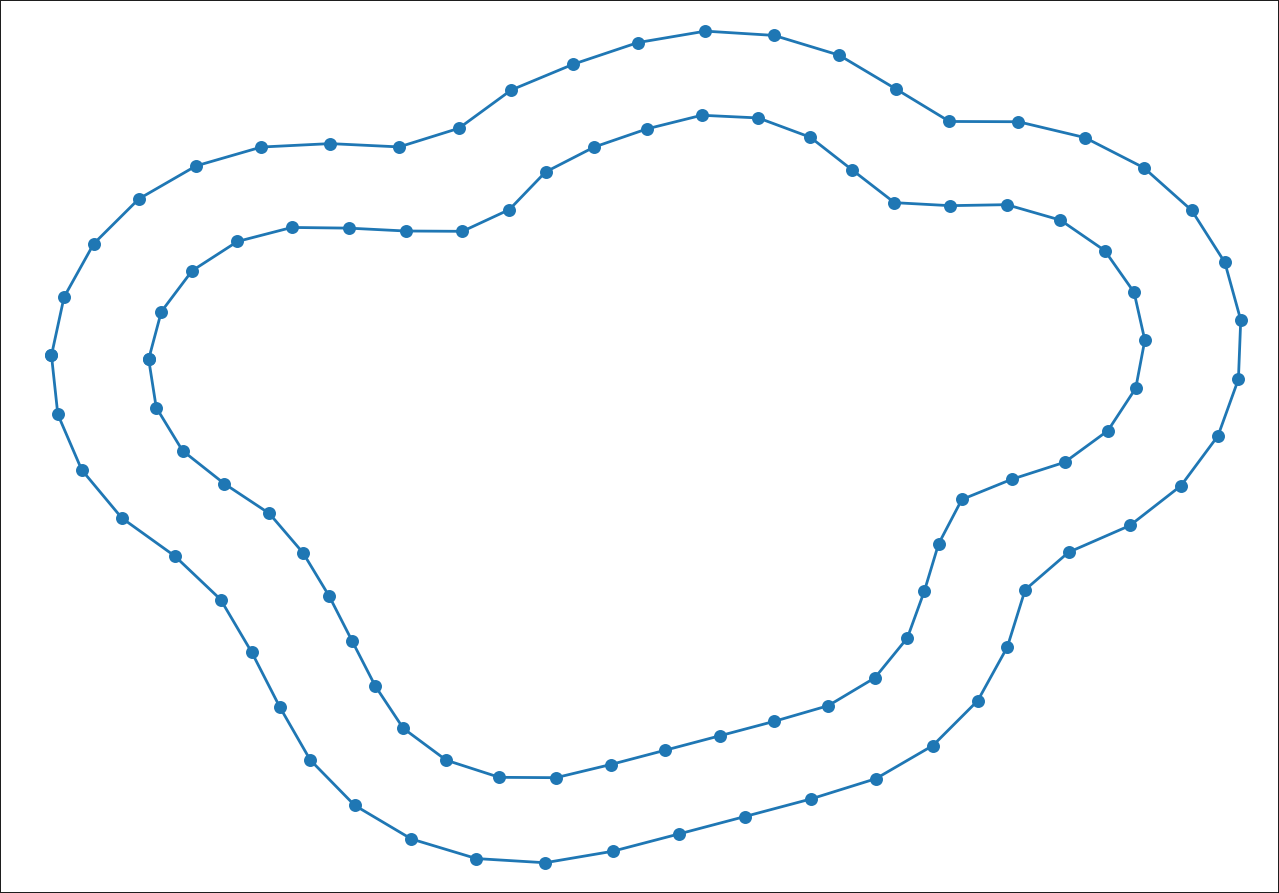
\includegraphics[width=\columnwidth]{track.png}}
			\caption{The generated track boundaries using the RNG seed 42. Blue dots mark the positions of cones.}
			\label{fig:track}
		\end{center}
		\vskip -0.2in
	\end{figure}
\end{frame}

\begin{frame}
	\frametitle{Tests}
\end{frame}

\begin{frame}
	\frametitle{Challenges}
\end{frame}

\begin{frame}
	\frametitle{outcome}
\end{frame}

\begin{frame}
	\frametitle{Reflection}
\end{frame}

\begin{frame}
	\frametitle{References}
\end{frame}

\end{document}